\documentclass{sig-alternate-05-2015}

% \usepackage{subfigure}
\usepackage{subfig}

\usepackage{balance}
\usepackage{multirow}
\usepackage{color}
\usepackage{chngpage}
\usepackage{url}
\usepackage{amsmath}
\usepackage{caption}
\usepackage{algorithm}
\usepackage{algpseudocode}
\usepackage{hyperref}

\newtheorem{theorem}{Theorem}[section]

\newcommand{\para}[1]{{\vspace{2pt} \bf \noindent #1 \hspace{8pt}}}

\newenvironment{packed_itemize}{
\begin{itemize}

}{\end{itemize}}


\makeatletter
\def\@copyrightspace{\relax}
\makeatother

\begin{document}

\captionsetup[subfigure]{labelformat=empty}

\title{Gaussian Process Regression}
\subtitle{A practical overview}
\author{
    \alignauthor \color{blue}\href{http://lzhbrian.me}{Tzu-Heng Lin}\color{black}, 2014011054, W42\\
    \affaddr{Department of Electronic Engineering, Tsinghua
      University, Beijing, China\\}
    \email{\color{blue}\href{mailto:lzhbrian@gmail.com}{lzhbrian@gmail.com}}
}


\maketitle
\begin{abstract}
\footnote{\color{blue}\href{http://lzhbrian.me}{Tzu-Heng Lin} \color{black} is currently an undergraduate student in the Department of Electronic Engineering, Tsinghua University. His research interests include Big Data Mining, Machine Learning, etc. For more information about me, please see \color{blue}\href{http://lzhbrian.me}{my personal website}\color{black}.
Please feel free to contact me at any time via \color{blue}\href{mailto:lzhbrian@gmail.com}{email} }Gaussian Process Regression(GPR) is a powerful, nonparametric tool developed based on the Bayesian theory and the Statistical learning theory. Choosing the right \emph{Mean Functions}, \emph{Kernel Functions} as well as the \emph{Likelihood Functions} and the \emph{Inference Methods} have been critical to the performance of the model. However, these works are often hard and require much expertise \& experience.

In this paper, we first give an introduction on the overall process of GPR. 
Subsequently, we give a precise explanation on some of the recent works which emphasize on the choice of the \emph{Kernel Function}.
In addition, we implement sufficient number of experiments to systematically analyze the performance of GPR with different \emph{Likelihood Functions} and the \emph{Inference Methods}. Our experiments are conducted on two interesting datasets. The best MSE we get from two experiments are 0.2112 \& 0.0262.

We seek to provide an comprehensive practical overview in the field of Gaussian Process Regression.

\end{abstract}




%
%  Use this command to print the description
%
\printccsdesc


\section{Introduction} \label{sec:introduction}

Machine learning has been a heated research topic these days. With this amazing tool, we are now capable of predicting the price of the stock price based on history, doing the classifying by just inputing the pixels of images.

Supervised learning is one of the most important sections for machine learning. And Regression is possibly the core of supervised learning.

In Gaussian Process Regression, we take advantage of the flexibility and simplicity of Gaussian Process and implement it into a regression problem. 


The structure of this pape is as follows: 
In section \ref{sec:intro} we provide an overview of Gaussian Process Regression. 
Section \ref{sec:autokernel} describes some of the recent works on the methods for auto-construction of the kernels.
In section \ref{sec:experiment} we conduct two experiments.
Conclusions are drawn in section \ref{sec:conclusion}.



% Section: Gaussian Process Regression
\section{Gaussian Process Regression} \label{sec:intro}

\subsection{Regression}

\para{Regression}
Regression is probably one of the most fundamental problems in a wide range of fields including \emph{Statistics}, \emph{Signal Processing} and \emph{Machine Learning}, etc. A regression problem is usually formulated as follows:
Given a training set $D = \{ (\textbf{x}_{i}, y_{i}) | i = 1,2,...,n \}$, we assume that $\textbf{x}_{i}, y_{i}$ have the following relationship:
	\begin{equation}
		y_{i} = f(\textbf{x}_{i}) + e
	\end{equation}
where $e$ is the error noise. By finding such $f(\cdot)$, we can predict what a corresponding $y^{*}$ is in some test case $\textbf{x}^{*}$. Note that $\textbf{x}$ can either be a vector or a scalar.

\para{Generalized Linear Model}
A widely used regression model is called Generalized Linear Model(GLM)\cite{mccullagh1984generalized}, in which a regression function can be expressed as a linear combination:
	\begin{equation}
		f(\textbf{x}) = \sum_{i=1}^{M} w_{i}\phi_i (\textbf{x})
	\end{equation}
where $\phi_{i}(x)$ is called the basis function.
In a regular GLM analysis, we have to firstly determine what our basis functions we are going to use, and subsequently can we use the training dataset to derive the parameters in the basis functions and the coefficients in the regression function.
	
\para{Mean Square Error}
We use a measurement called the Mean Square Error(MSE) to evaluate the performance of the regression function. It is defined as follows:
	\begin{equation}
		MSE = \frac{1}{m}\sum^{m}_{i=1} (f(\textbf{x}^{*})-y_{i}^{*})^{2}
	\end{equation}
where $f(x)$ represents the regression function. A smaller MSE represents a better regression function on a test set.


\subsection{Gaussian Process Regression}

\para{Gaussian Process}
A Gaussian Process(GP) is any distribution over functions such that any finite set of function values $f(x_1), f(x_2), ..., f(x_N)$ have a joint Gaussian distribution\cite{rasmussen2006gaussian}. It can usually be represented as
\begin{equation}
N\{ E[ f(x) ], Cov[f(x), f(x^{'})] \}
\end{equation}
where $E[ f(x) ]$ refers to its \emph{Mean Function}, and $Cov[f(x), f(x^{'})]$ refers to its \emph{Covariance Function}.

\para{Gaussian Process Regression}
Gauss Process Regression(GPR)\cite{rasmussen2006gaussian} is a popular regression method these years.
The key of this method is to model the regression function $\{ f(\textbf{x}) | \textbf{x} \in S\}$ as a GP 
\begin{equation}
f(x) \gets N \{ m(\textbf{x}), K (\textbf{x},\textbf{x}^{'}) \}
\end{equation}
where $m(\textbf{x})$ is the \emph{Mean function} and $K (\textbf{x},\textbf{x}^{'})$ is the \emph{Kernel Function}.

In a GPR, we don't have to derive the exact form of the regression function, we just need to determine the form of the above two functions. 
As introduced in GP, the \emph{Kernel Function} $K (\textbf{x},\textbf{x}^{'})$ is actually the covariance between $f(\textbf{x})$ and $f(\textbf{x}^{'})$, and if it is a zero-mean GP, the covariance turns into correlation. So a \emph{Kernel Function} represents the relationship between $f(\textbf{x})$ and $f(\textbf{x}^{'})$.

By calculating the posterior probability of the desired $f(\textbf{x}^{*})$, \emph{i.e.} $p(f(\textbf{x}^{*}) | \textbf{x}^{*}, D)$, we can derive the mean value along with the standard deviation of this estimation. 
On the other hand, we must noted that calculating the posterior probability will become an intractable work when we have a high-dimensional dataset. It is a need that we introduce some inference method to estimate this work. \\

To summarize, choosing a suitable \emph{Mean Functions}, \emph{Kernel Functions} as well as the \emph{Likelihood Functions} and the \emph{Inference Methods} is the key of a GPR model.
Rasmussen's \emph{Gaussian Processes for Machine Learning}\cite{rasmussen2006gaussian} has implemented some marvellous Matlab/Octave code of GPR, it is available on his website\footnote{Available at \color{blue}\href{http://www.gaussianprocess.org/gpml/code/matlab/doc/}{http://www.gaussianprocess.org/gpml/code/}} known as \textbf{\emph{GPML}}.




% Section: Related Work
\section{Related Work} \label{sec:related}

\para{Kernel Function}


\para{Inference Methods}
Some popular works on inference methods include
MCMC\cite{gamerman1997sampling},
Expectation Propagation\cite{minka2001expectation},
Variational Bayes\cite{palmer2006variational,nickisch2009convex}
and Laplace Approximation\cite{tierney1986accurate},
etc.
Due to the limited time and space, we won't go very deep into these inference methods.

% Section: Kernel
\section{Kernel choice} \label{sec:autokernel}
Choosing an appropriate \emph{Kernel Function} in a regression problem has always been a nightmare for researchers and analysts. In this section, from the practical meaning of a \emph{Kernel Function}, we introduce an automatic way to construct a desired composite form of \emph{Kernel}.
We also introduce a special \emph{Additive Kernel} used specifically for an Additive Gaussian Process, which is a case we will be solving in our experiment (Section~\ref{sec:experiment}).
This section is based on the work of Duvenaud and Lloyd et. al \cite{duvenaud2013structure,lloyd2014automatic,duvenaud2014automatic,duvenaud2011additive}.


\subsection{Kernels express structures}

%% Base Kernels

\para{Base Kernels}
As we all know, different kernels can represent different kinds of data. In Figure~\ref{fig:singlekernel}, we show 4 different kinds of base kernels, each represents a specific kind of data characteristics (Table~\ref{tab:kernel}). Each function of the kernel is shown in Equation~\ref{eqa:kernel}


\begin{equation}
\left \{
\begin{aligned} \label{eqa:kernel}
k_{LIN}(x,x^{'}) &= \sigma_{b}^{2} + \sigma_{v}^{2} (x-l)(x^{'}-l) 	\\
k_{SE}(x,x^{'}) &= \sigma^2 exp(-\frac{(x-x^{'})^2}{2l^2})	\\
k_{PER}(x,x^{'}) &= \sigma^2 exp(-\frac{2sin^2 (\pi(x-x^{'})/p)}{l^2})	\\
k_{RQ}(x,x^{'}) &= \sigma^2 (1+\frac{(x-x^{'})^2}{2\alpha l^2})^{-\alpha}	\\
\end{aligned}
\right.
\end{equation}


\begin{figure}[htp]
\begin{minipage}[htp]{1\linewidth}
	\centering
  	\subfloat[Linear(LIN)]{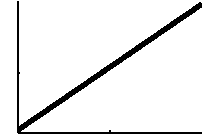
\includegraphics[width=0.45\textwidth]{figure/kernels/lin_kernel.pdf}}
	\subfloat[Squared exp(SE)]{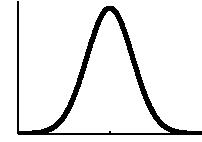
\includegraphics[width=0.45\textwidth]{figure/kernels/se_kernel.pdf}}\\
	\subfloat[Periodic(PER)]{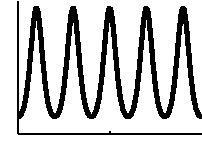
\includegraphics[width=0.45\textwidth]{figure/kernels/per_kernel.pdf}}
	\subfloat[Rational quadratic(RQ)]{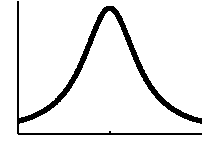
\includegraphics[width=0.45\textwidth]{figure/kernels/rq_kernel.pdf}}
% \vspace{-0.1in}
\caption{Base Kernels}
\label{fig:singlekernel} % FIG1
\end{minipage}
\vspace{-0.05in}
\end{figure}


\begin{table}[htp]
\centering
{\small
\begin{tabular}{c|c}
    \hline
    \textbf{Kernel} & \textbf{Data Structures} \\ 
    \hline
	   Linear(LIN) & linear functions\\
	   Squared exponential(SE) & local variation\\
	   Periodic(PER) & repeating structure\\
	   Rational quadratic(RQ) & multi-scale variation\\
	   \hline
\end{tabular}
}
\caption{Different kinds of kernels and its represented data structures.}
\label{tab:kernel}
% \vspace{-0.05in}
\end{table}



%% Compositional Kernels
\para{Compositional Kernels}
When the data structure we are dealing with is not contained in any of the above base kernel, we have to made one to fit the targeted data characteristics. A possible and probable approach of making a customized kernel is to do some addition and multiplication to the base kernels.
\begin{align}
k_{k_{a} + k_{b}} (\textbf{x}, \textbf{x}^{'}) &= k_{a} (\textbf{x}, \textbf{x}^{'}) + k_{b} (\textbf{x}, \textbf{x}^{'}) \\
k_{k_{a} \times k_{b}} (\textbf{x}, \textbf{x}^{'}) &= k_{a} (\textbf{x}, \textbf{x}^{'}) \times k_{b} (\textbf{x}, \textbf{x}^{'})
\end{align}
By addition and multiplication, we are able to construct some very complicated data structure.
Below, we show some examples of structures by compositional kernels (Figure~\ref{fig:compKernel}) and the data structures they are capable of representing (Table~\ref{tab:compKernel}).


\begin{figure}[htp]
\begin{minipage}[htp]{1\linewidth}
	\centering
  	\subfloat[LIN + PER]{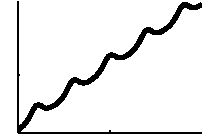
\includegraphics[width=0.45\textwidth]{figure/kernels/lin_plus_per.pdf}}
	\subfloat[SE + PER]{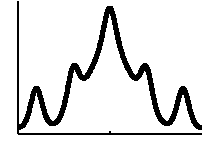
\includegraphics[width=0.45\textwidth]{figure/kernels/se_plus_per.pdf}}\\
	\subfloat[SE $\times$ PER]{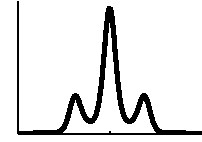
\includegraphics[width=0.45\textwidth]{figure/kernels/se_times_per.pdf}}
	\subfloat[LIN $\times$ LIN]{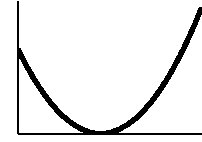
\includegraphics[width=0.45\textwidth]{figure/kernels/lin_times_lin.pdf}}
% \vspace{-0.1in}
\caption{Some examples of the compositional kernels}
\label{fig:compKernel} % FIG1
\end{minipage}
\vspace{-0.05in}
\end{figure}


\begin{table}[htp]
\centering
{\small
\begin{tabular}{c|c}
    \hline
    \textbf{Kernel} & \textbf{Data Structures} \\ 
    \hline
	   LIN+ PER & periodic plus trend\\
	   SE + PER & periodic plus noise\\
	   SE $\times$ PER & locally periodic\\
	   LIN $\times$ LIN & quadratic functions\\
	   \hline
\end{tabular}
}
\caption{Some examples of the compositional kernels}
\label{tab:compKernel}
% \vspace{-0.05in}
\end{table}


\subsection{Automatic Construction} \label{sec:autokernel}
As we can see in the above analysis, choice of the form of a \emph{Kernel Function} can be critical in a GPR. However, this process was used to be a privileged work for experts since it requires a whole lot of experience and expertise. In \cite{duvenaud2013structure,lloyd2014automatic,duvenaud2014automatic}, Duvenaud and Lloyd et.al describe a tractable method to let a computer be capable of doing this work.
This procedure is summarized as follows:

\para{Kernel Family}
We consider the \emph{base kernels} as shown in Figure~\ref{fig:singlekernel}, any algebraic expression using these kernels as a combination of $+$ and $\times$ could be our target. And any of our target with the concatenation of the parameters forms a kernel family.

\para{Scoring a Kernel Family}
We must find a way to evaluate a kernel family. At here, we use the marginal likelihood\cite{blumer1987occam} as our criterion, and use the Bayesian Information Criterion(BIC)\cite{schwarz1978estimating} to approximate the integration over kernel parameters.

\para{Search over structures}
Last, by using a greedy search: At each stage, expand the current kernel by all possible \emph{operators}
and choose the highest scoring one. The number of working stage is defined by user.
Possible operators are listed as follows:
\begin{enumerate}
	\item Any expression $S$ can be replaced by $S + B$
	\item Any expression $S$ can be replaced by $S \times B$
	\item Any base kernel $B$ can be replaced by $B^{'}$
\end{enumerate}
where $B$ and $B^{'}$ represent any base kernel family. Note that, in the work \cite{lloyd2014automatic}, Lloyd et. al also take account of the changepoint operator $CP$, the changewindow operator $CW$, and some empirical operators. They also add some base kernels to improve the algorithm. Due to limited time and space, we only introduce the most important part here.

The implemented Matlab and Python code by Duvenaud and Lloyd et.al can be found on github\footnote{Available at \color{blue}\href{http://github.com/jamesrobertlloyd/gpss-research}{github.com/jamesrobertlloyd/gpss-research} \color{black} and \color{blue}\href{http://github.com/jamesrobertlloyd/gp-structure-search}{github.com/jamesrobertlloyd/gp-structure-search}.}.

\begin{algorithm}[t]
        \caption{Automatic kernel construction algorithm}
        \begin{algorithmic}
        		\Require Required search depth $N$
        		\State Initialize kernel $S$
            	\For{$t = 1 \to N$}
			\State $CurScore \gets 0$
			\For{$ Possible ~ operators ~ S^{'}$}
	            		\If {Score(S) > CurScore}
					\State $S \gets S^{'}$
				\EndIf
			\EndFor
	    	\EndFor
		\State \Return $kernel~S$
       	\end{algorithmic}
\end{algorithm}


\subsection{Additive Gaussian Processes}

\para{Additive Gaussian Process}
\cite{duvenaud2011additive}
In some 


\para{Additive Kernels}
We now give the precise definition of additive kernels.
As shown in \cite{duvenaud2011additive}, we define the 1st, 2nd, nth order additive kernel as:
\begin{align}
k_{add_{1}} (\textbf{x},\textbf{x}^{'}) &= \sigma^2_1 \sum_{i=1}^{D} k_{i} (\textbf{x}_{i},\textbf{x}_{i}^{'}) \\
k_{add_{2}} (\textbf{x},\textbf{x}^{'}) &= \sigma^2_2 \sum_{i=1}^{D} \sum_{j=i+1}^{D} k_{i} (\textbf{x}_{i},\textbf{x}_{i}^{'}) k_{j} (\textbf{x}_{j},\textbf{x}_{j}^{'}) \\
k_{add_{n}} (\textbf{x},\textbf{x}^{'}) &= \sigma^2_n \sum_{1 \leqslant i_1 < i_2 < ... < i_n \leqslant D} ( \prod_{d=1}^{n} k_{i_d} (\textbf{x}_{i_d},\textbf{x}_{i_d}^{'}) ) \\
\end{align}
where $k_{i} (\textbf{x}_{i},\textbf{x}_{i}^{'})$ is the \emph{base kernel} we assigned at first for each dimension $i \in \{1,2,...,D\}$.
A full additive kernel is a sum of all orders' additive kernels, as in equation~\ref{eqa:add}:
\begin{equation} \label{eqa:add}
K_{add_{full}} (\textbf{x},\textbf{x}^{'}) = \sum_{n=1}^{D} k_{add_{n}} (\textbf{x},\textbf{x}^{'})
\end{equation}
In the real practice, we could choose specific orders of the additive kernels:
\begin{equation} \label{eqa:add}
K_{add_{prac}} (\textbf{x},\textbf{x}^{'}) = \sum_{n} k_{add_{n}} (\textbf{x},\textbf{x}^{'})
\end{equation}

We also noted that if every base kernel is a one-dimensional squared-exponential(SE) kernal, the Dth order term of the additive kernel would be:
\begin{equation} \label{eqa:add}
\begin{aligned}
K_{add_{D}} (\textbf{x},\textbf{x}^{'}) &= \sigma_{D}^{2} \prod_{d=1}^D k_{d} (\textbf{x}_{d},\textbf{x}_{d}^{'}) \\
		     &= \sigma_{D}^{2} \prod_{d=1}^D exp(-\frac{(\textbf{x}_{d}-\textbf{x}_{d}^{'})^{2}}{2l_{d}^{2}}) \\
		     &= \sigma_{D}^{2}  exp(-\sum_{d=1}^{D} \frac{(\textbf{x}_{d}-\textbf{x}_{d}^{'})^{2}}{2l_{d}^{2}})
\end{aligned}
\end{equation}
which is just the multivariate squared-exponential kernel.

















% Section: Experiments
\section{Experiments} \label{sec:experiment}


%% First
\subsection{First Experiment}
Our first experiment is conducted on a one-dimensional data as shown in Figure~\ref{fig:data1}. In this experiment, we have a 543-point training set ranging from $x = -32$ to $x = 14$, and we want to predict some 67-point test set ranging from $x = 14$ to $x = 21$.

\begin{figure}[htp]
\begin{minipage}[htp]{1\linewidth}
	\centering
  	\subfloat{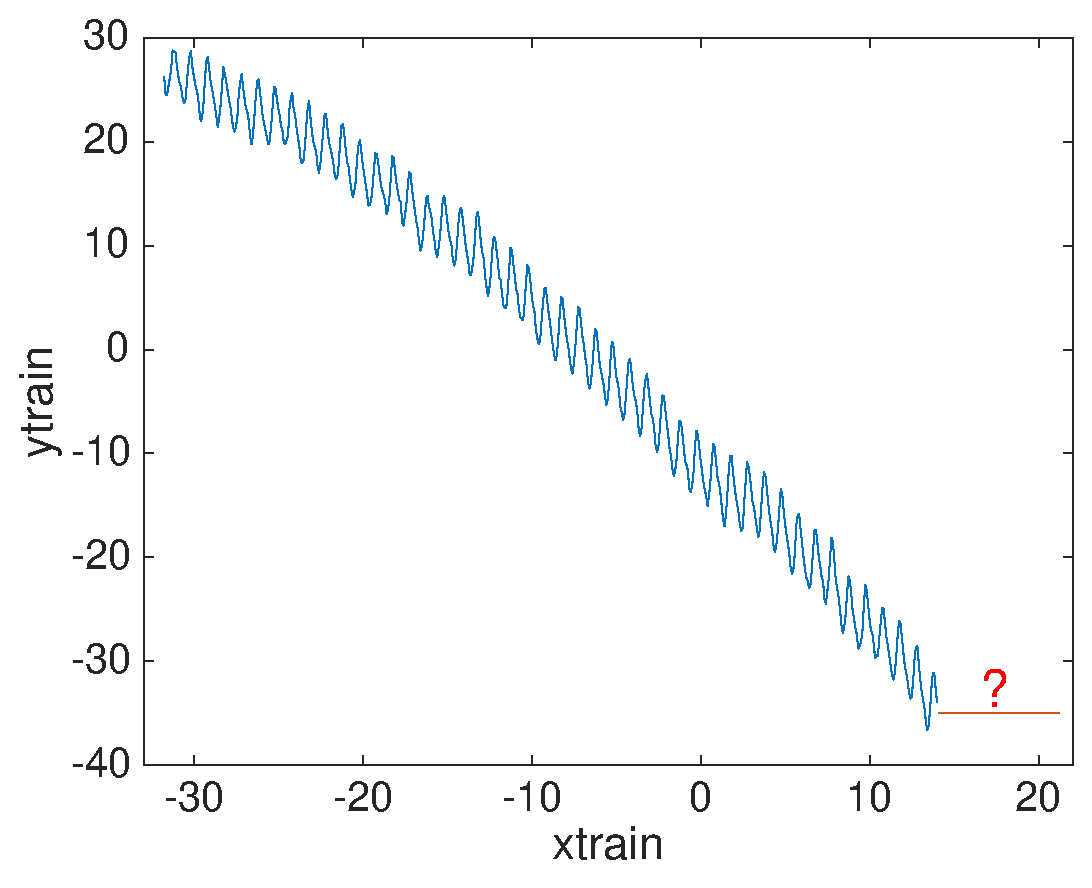
\includegraphics[width=0.7\textwidth]{figure/data1.eps}}
% \vspace{-0.1in}
\caption{A one-dimensional dataset}
\label{fig:data1} % FIG1
\end{minipage}
\vspace{-0.05in}
\end{figure}

To better do this work, we use the Auto Construction Kernel method described in Section~\ref{sec:autokernel}.
By doing a lengthy greedy kernel construction procedure, we derive a compositional kernel:
\begin{equation}
LIN \times SE + SE \times ( PER + RQ )
\end{equation}
And by using the Guassian Likelihood function and the exact posterior probability.
We predict the results as in Figure~\ref{fig:predict1}

\begin{figure}[htp]
\begin{minipage}[htp]{1\linewidth}
	\centering
  	\subfloat{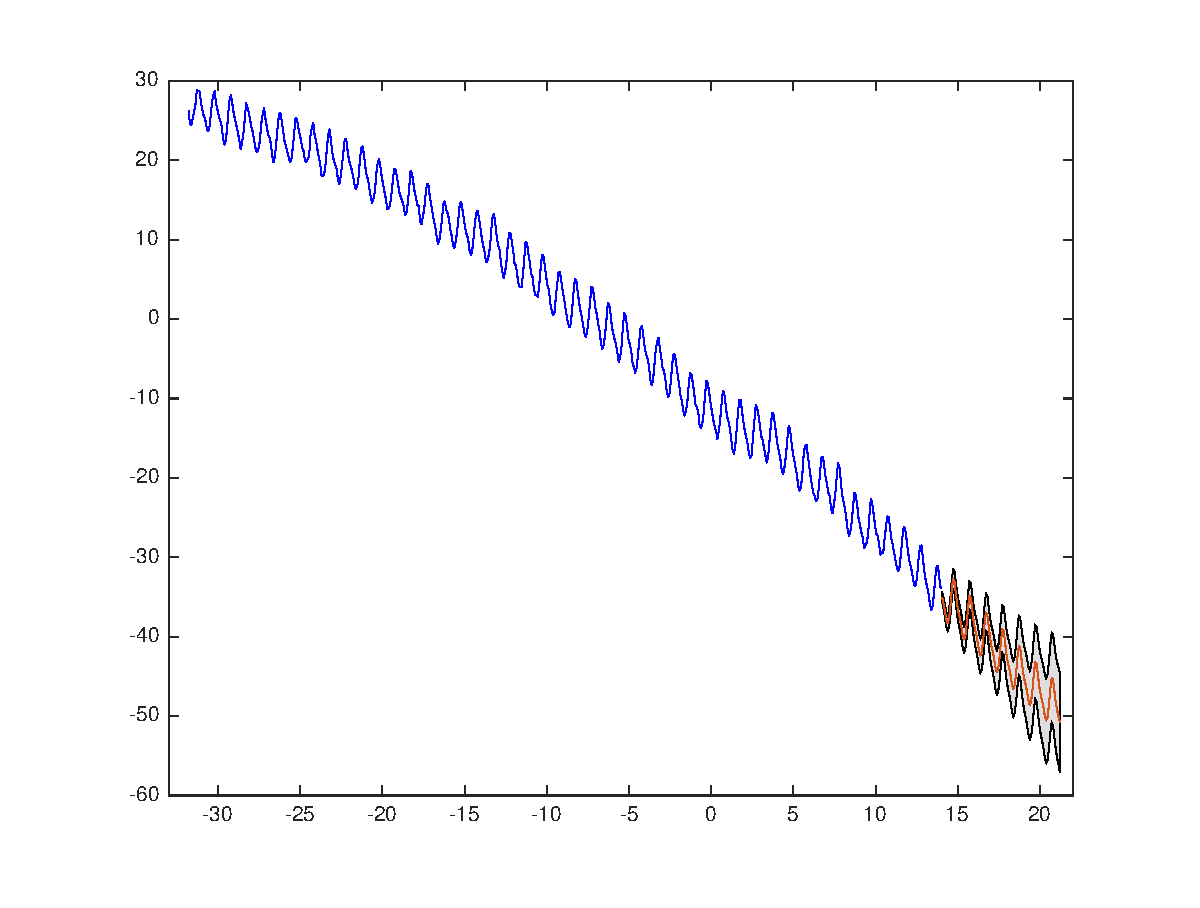
\includegraphics[width=0.7\textwidth]{figure/predict1.eps}}
% \vspace{-0.1in}
\caption{Prediction of the 1st dataset}
\label{fig:predict1} % FIG1
\end{minipage}
\vspace{-0.05in}
\end{figure}

We could achieve an \textbf{MSE} of \textbf{0.2112} using this method. Given that the output data ranges from $-60 - 30$, we believe that we have a satisfying result.



%% Second
\subsection{Second Experiment}

\begin{figure}[htp]
\begin{minipage}[htp]{1\linewidth}
	\centering
  	\subfloat{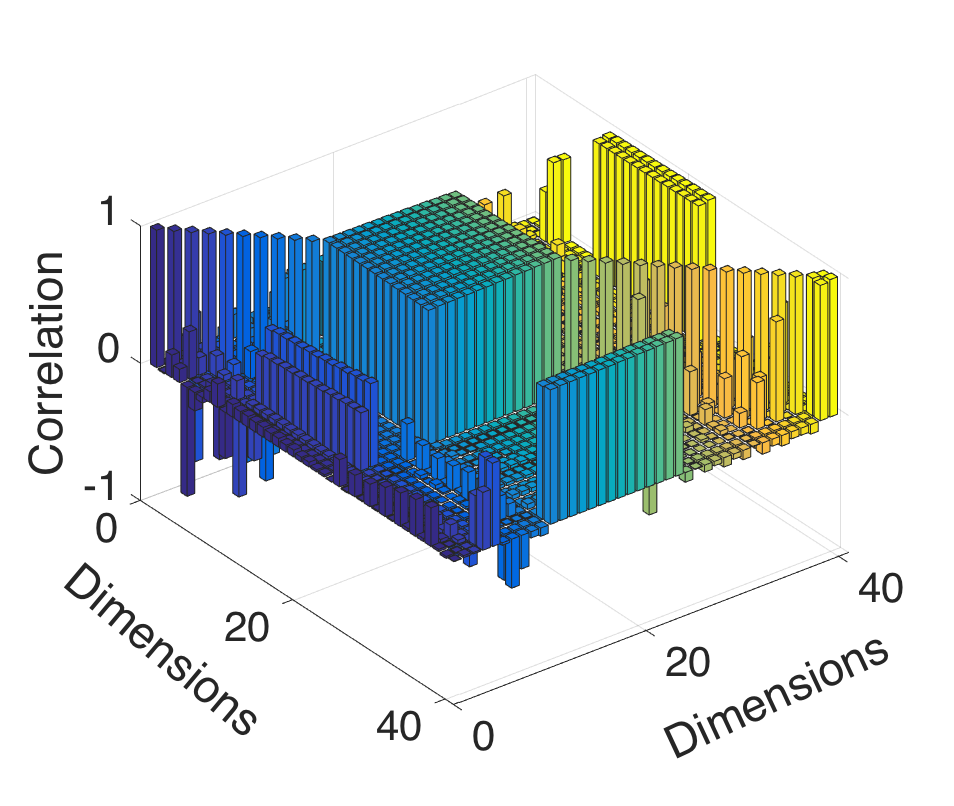
\includegraphics[width=0.9\textwidth]{figure/data2.eps}}
% \vspace{-0.1in}
\caption{A 40-dimensional dataset, Correlation between each dimension of \textbf{x}}
\label{fig:data2}
\end{minipage}
\vspace{-0.05in}
\end{figure}

\para{Dataset}
Given a such high-dimensional dataset, we decide to first analyze the relationship between each dimension.
As shown in Figure~\ref{fig:data2}, we can see that actually 16 dimensions of the 40-dimensional \textbf{x} are highly correlated to each other (correlation > 0.96).
So reducing the dimension of this dataset is a probable way to reduce the complexity of the algorithm.
Thus, we do this procedure by ignoring the \{12:24, 25:38\} dimensions, which are all highly correlated to the 11th dimension. And we consequently derive a 25-dimensional set.


%%% ABCD
\subsubsection{Auto Construction}
By conducting a greedy kernel search as in the previous experiment, we get a desired kernel function: \emph{SE}.

We hereby use this dataset to test the performance of different \emph{Likelihood Functions} and \emph{Inference Methods}.

\begin{table}[h]
\centering
{\small
\begin{tabular}{|c|cccc|}
    \hline
	    & exact & Laplace & VB & L00 \\ 
    \hline
	   Gaussian & & & & \\
	   Laplace & & & & \\
    \hline
\end{tabular}
}
\caption{MSE using different kinds of \emph{Likelihood Functions} and \emph{Inference Methods}. Different rows represents different \emph{Likelihood Functions} and different columns represents different \emph{Inference Methods}. }
\label{tab:predict21}
% \vspace{-0.05in}
\end{table}



%%% Additive Gaussian
\subsubsection{Additive Kernel}

%%%%
\para{Dataset Structure}
We surprisingly found that each dimension is gauss

%%%%
\para{Additive Kernel}
Since we have a 25-dimension(reduced) dataset, we set the kernel functions as:
\begin{equation}
\begin{aligned}
K_{add} &= \sum_{r=1}^{R} k_{add_{r}} (\textbf{x},\textbf{x}^{'}) \\
 &= \sum_{r=1}^{R} \{ \sigma^2_r \sum_{1 \leqslant i_1 < i_2 < ... < i_r \leqslant D} ( \prod_{d=1}^{r} k_{i_d} (\textbf{x}_{i_d},\textbf{x}_{i_d}^{'}) ) \}
\end{aligned}
\end{equation}
where 
\begin{equation}
k_{i_d} (\textbf{x}_{i_d},\textbf{x}_{i_d}^{'}) = SE = exp(-\frac{(\textbf{x}_{i_d}-\textbf{x}_{i_d}^{'})^{2}}{2l_{i_d}^{2}})
\end{equation}
We also use the same analysis method as in the last subsubsection, the result is shown in Table~\ref{tab:predict22}.

\begin{table}[h]
\centering
{\small
\begin{tabular}{|c|cccc|}
    \hline
	    & exact & Laplace & VB & L00 \\ 
    \hline
	   Gaussian & & & & \\
	   Laplace & & & & \\
    \hline
\end{tabular}
}
\caption{MSE using different kinds of \emph{Likelihood Functions} and \emph{Inference Methods}. Different rows represents different \emph{Likelihood Functions} and different columns represents different \emph{Inference Methods}. }
\label{tab:predict22}
% \vspace{-0.05in}
\end{table}












% Section: Conclusion
\section{Conclusion} \label{sec:conclusion}
In this paper, we discuss about the Gaussian Process Regression.
We comprehensively introduce the concept of Gaussian Process Regression.
Specifically, we precisely explain the recent works for kernel auto construction.
We also conduct two experiments, in which we systematically compare the performance of two Likelihood Functions and three Inference Methods. 
\textbf{The best MSE we get from two experiments are 0.2112 \& 0.0262.}

As future work, we would like to join more information of GPR to this paper such as the details of how a hyperparameter is derived and some deeper discussion about the Inference methods; and if could, propose some improvement to the algorithms available.


% Last
\renewcommand{\baselinestretch}{1.1}
\balance
% \small
% Acknowledgement
\section{Acknowledgement} \label{sec:acknowledgement}
I would like to thank Yuanxin Zhang, XueChao Wang, for the discussion with me on the algorithms. Without them, I wouldn't have the possibility to accomplish this work in such a short time. This paper is a project of Stochastic Process Course in Tsinghua University, taught by Prof. Zhijian Ou.\\

\para{Source Code and Dataset} Source Code to perform all experiments, along with the dataset in this paper can be found in my github repository\footnote{Available at \color{blue}\href{http://github.com/lzhbrian/gpr}{http://github.com/lzhbrian/gpr}}. Due to my limited knowledge, there might be some mistakes and flaws in this paper as well as in the code, please do not hesitate to contact and correct me.


% Reference
\bibliographystyle{abbrv}
\bibliography{ref}


\end{document}

